\section{Durchführung}
\label{sec:Durchführung}

\begin{figure}[H]
  \centering
  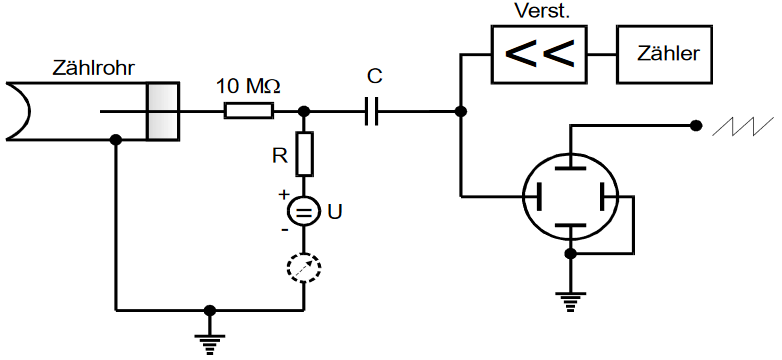
\includegraphics[height=5cm]{Schaltung.PNG}
  \caption{Aufbau der Messapparatur \cite{sample}.}
  \label{fig:schaltung}
\end{figure}

Der Versuch wird mit einer Schaltung gemäß Abbildung \ref{fig:schaltung} durchgeführt.
Der durch die Ionisation im Zählrohr entstehende Spannungsimpuls wird dabei über den Kondensator
ausgekoppelt und kann schließlich nach Verzögerung im Verstärker mit dem Zählgerät registriert
oder alternativ auf dem Bildschirm des Oszilloskops graphisch dargestellt werden.

Zum Aufnehmen der Charakteristik des Zählrohrs wird vor dieses eine $\beta$-Strahlungsquelle gesetzt.
Bei unterschiedlichen Spannungen zwischen dessen Anode und Kathode (Bereich 300-700 V) wird nun die
Zählrate gemessen. Dies geschieht jeweils über einen Zeitraum von 60 Sekunden. Zudem wird bei jeder
Spannung auch die entsprechend entstehende Stromstärke am Geiger-Müller-Zählrohr abgelesen.

Anschließend werden die Spannungsimpulse auf dem Oszilloskops dargestellt. Da dabei in etwa ein
Bild entsprechend Abbildung \ref{fig:totzeit} entsteht, lassen sich Totzeit und Erholungszeit
ungefähr mit dem Auge ablesen.

Zuletzt wird dann, wieder mit dem Zählgerät, die Zwei-Quellen-Messung durchgeführt.
Dabei wird als Erstes die Zählrate von lediglich einer Strahlungsquelle über einen Zeitraum
von diesmal 120 Sekunden gemessen. Danach wird eine zweite Quelle hinzugefügt und die Messung
exakt gleich wiederholt. Schließlich wird die Messung ein drittes mal allein für die
als zweites hinzugefügte Quelle durchgeführt, sodass man letztendlich drei unterschiedliche
Zählraten gemessen hat (Quelle 1, Quelle 2, Quelle 1 und 2).
